\documentclass[aspectratio=169]{beamer}
\usetheme[block=fill]{metropolis}
\usepackage{tikz}
\usetikzlibrary{shapes.geometric, arrows.meta, positioning, calc}

\title{Building a Reproducible Scholarly Search Toolkit}
\subtitle{Episode 18: File System Export \& Reporting}
\author{Scholar Search Kit}
\date{}

\begin{document}

\begin{frame}[plain]
  \titlepage
\end{frame}

\begin{frame}{Episode Goal}
  \begin{alertblock}{The Goal}
    Create a structured \texttt{RunReport} that captures execution metadata and writes outputs to safely namespaced directories.
  \end{alertblock}
  \vspace{0.5cm}
  If a researcher runs 5 different queries, they need to know which file belongs to which query. We must generate timestamped, uniquely named folders for every execution.
\end{frame}

\begin{frame}{The Output Architecture}
  \begin{center}
  \resizebox{0.7\linewidth}{!}{
  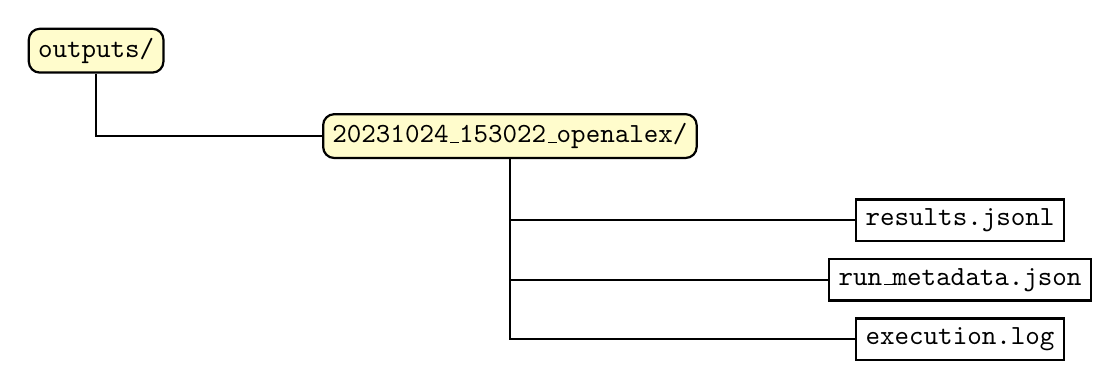
\begin{tikzpicture}[
      node distance=0.5cm and 2cm,
      folder/.style={rectangle, draw, thick, rounded corners, fill=yellow!20, align=left},
      file/.style={rectangle, draw, thick, fill=white, align=left},
      arrow/.style={-{Stealth[scale=1.2]}, thick}
    ]
    
    \node[folder] (root) {\texttt{outputs/}};
    \node[folder, below right=of root] (run) {\texttt{20231024\_153022\_openalex/}};
    
    \node[file, below right=of run] (data) {\texttt{results.jsonl}};
    \node[file, below=0.2cm of data] (meta) {\texttt{run\_metadata.json}};
    \node[file, below=0.2cm of meta] (log) {\texttt{execution.log}};
    
    \draw[thick] (root.south) |- (run.west);
    \draw[thick] (run.south) |- (data.west);
    \draw[thick] (run.south) |- (meta.west);
    \draw[thick] (run.south) |- (log.west);
  \end{tikzpicture}
  }
  \end{center}
  \vspace{0.2cm}
  Every execution gets a sealed envelope containing the data, the logs, and exactly what parameters were used.
\end{frame}

\begin{frame}{Implementation: \texttt{RunReport}}
  \begin{block}{Reproducibility}
    Science requires reproducibility. You must be able to prove \textit{exactly} what you searched for six months later.
  \end{block}
  
  \begin{itemize}
      \item The \texttt{RunReport} saves the exact query string, the provider used, the timestamp, and the final document count.
      \item It acts as the "receipt" for the data extraction phase.
  \end{itemize}
\end{frame}

\begin{frame}{Safe Path Generation}
  \begin{block}{Cross-Platform Paths}
    Windows uses \texttt{\\}, Mac/Linux use \texttt{/}.
  \end{block}
  
  \begin{itemize}
      \item We use Python's \texttt{pathlib.Path} to ensure directories are created safely across all operating systems.
      \item We sanitize queries (removing spaces and special characters) before using them in folder names.
  \end{itemize}
\end{frame}

\begin{frame}{Verification}
  \begin{alertblock}{Success Criteria}
    \begin{itemize}
        \item Running the CLI automatically creates an \texttt{outputs/} directory.
        \item A timestamped subfolder is created containing both the results and a \texttt{run\_metadata.json} file.
    \end{itemize}
  \end{alertblock}
\end{frame}

\end{document}
